\chapter{Introduction to Financial Data Science}
\label{chap:Introduction to Financial Data Science}

\begin{center}
\begin{tabular}{p{0.06\linewidth} | p{0.88\linewidth}}
	\toprule
	\multicolumn{2}{l}{\textbf{LEARNING OUTCOMES}} \\
	\midrule
	a & describe how big data, machine learning, and artificial intelligence are used in financial data science, fintech, and investment management \\
	\bottomrule
\end{tabular}
\end{center}

\vspace{1.5em}

\section{Financial Data and Big Data}
\label{sec:Financial Data and Big Data}

\textcolor{blue}{\textit{Dữ liệu định lượng (quantitative) như giá cả, lợi suất đã rất quen thuộc. Nhưng cuộc cách mạng thực sự nằm ở dữ liệu định tính (qualitative) và dữ liệu thay thế (alternative data). Nhờ sự phát triển của công nghệ số, chúng ta có thể chuyển hóa các cuộc gọi thu nhập, tin tức hay bài đăng mạng xã hội thành số liệu để phân tích đồng thời. Hãy suy nghĩ: dữ liệu nào sẽ mang lại lợi thế cạnh tranh lớn hơn trong tương lai?}}

\subsection{Quantitative vs. Qualitative Data}
The investment decision-making process analyzes both quantitative and qualitative data:
\begin{itemize}
	\item \textbf{Quantitative data} describes numeric information, such as prices, returns, interest rates, currency exchange rates, economic indicators, and accounting numbers, that can be analyzed using statistical methods.
	\item \textbf{Qualitative data} describes non-numeric information, such as market sentiment, management quality, industry trends, environmental factors (ESG), and geopolitical risks.
\end{itemize}
With the advance of digitization, qualitative data are increasingly captured digitally and processed algorithmically (e.g., using sentiment analysis), allowing for the integration of qualitative insights with quantitative analysis.

\subsection{Characteristics of Big Data (The 4 Vs)}
Datasets available for analysis are growing rapidly. Big data are characterized by four key dimensions:
\begin{itemize}
	\item \textbf{Volume:} The vast amount of data collected (ranging from megabytes to gigabytes, terabytes, and petabytes), representing millions or billions of observations.
	\item \textbf{Velocity:} The speed at which data are communicated and updated. Real-time or low-latency data feeds have become the standard in financial applications.
	\item \textbf{Variety:} The diversity of data formats and sources, which can be structured, semi-structured, or unstructured.
	\item \textbf{Veracity:} The credibility, authenticity, and reliability of different data sources. Veracity is critical in big data because of the varying quality of large, non-traditional datasets.
\end{itemize}

\begin{figure}[!htbp]
	\centering
	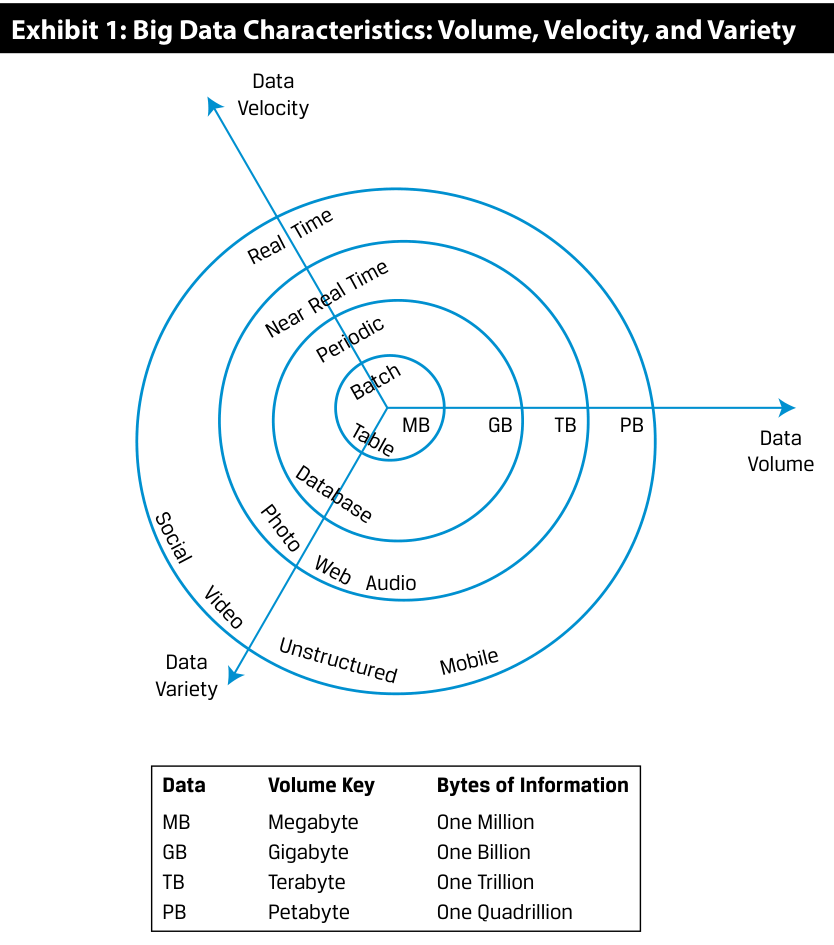
\includegraphics[width=0.75\linewidth]{002_figs/011_Module_11/11.1-Big Data Characteristics.png}
	\caption{Characteristics of Big Data: Volume, Variety, and Velocity}
	\label{fig:big_data_characteristics}
\end{figure}

\subsection{Data Types and Sources}
Data can be classified into three types based on structure:
\begin{itemize}
	\item \textbf{Structured data:} Organized in tables (rows and columns) and commonly stored in databases where fields are defined (e.g., SQL tables, CSV files).
	\item \textbf{Unstructured data:} Disparate, unorganized data that do not fit into traditional tables. Examples include social media posts, emails, voice recordings, pictures, and video feeds.
	\item \textbf{Semi-structured data:} Blends structured and unstructured elements. The data do not fit into traditional tables but contain tags or markers (e.g., HTML/XML code, JSON files, tagged financial news).
\end{itemize}

Table~\ref{tab:big_data_sources} outlines common sources of big data in finance:

\begin{table}[!htbp]
\centering
\caption{Examples of Big Data Sources in Finance}
\label{tab:big_data_sources}
\begin{tabular}{p{0.25\linewidth} | p{0.65\linewidth}}
	\toprule
	\textbf{Source} & \textbf{Examples} \\
	\midrule
	Financial markets & Equity, fixed income, futures, options, other derivatives, and commodities. \\
	Businesses & Corporate financial statements, commercial transactions, credit card purchases, and supply chain data. \\
	Governments & Trade, economic indicators, regulatory filings, taxation, and payroll data. \\
	Individuals & Personal websites, online product reviews, internet search logs, email, and social media posts. \\
	Sensors & Satellite imagery, aircraft tracking, shipping cargo data, and vehicle traffic patterns. \\
	Internet of Things & Data from smart buildings (climate control, energy usage) and connected commercial devices. \\
	\bottomrule
\end{tabular}
\end{table}

\subsection{Alternative Data and Risks}
\textbf{Alternative data} refers to information collected from non-traditional sources, such as satellite imagery, web traffic, social media sentiment, mobile device geolocation, and retail point-of-sale scanners.
\begin{itemize}
	\item \textbf{Data generated by individuals:} Personal activities like social media clicks, product reviews, and web searches. This data tends to be unstructured and qualitative.
	\item \textbf{Data generated by business processes:} Direct transactions like credit card purchases or point-of-sale scanner data. This structured data acts as a leading indicator of performance, whereas traditional corporate filings are lagging indicators.
	\item \textbf{Data generated by sensors:} Satellite imagery (e.g., counting cars in retail parking lots to predict earnings or monitoring flare gas at oil rigs) and Internet of Things (IoT) streams. It is largely unstructured and grows exponentially.
\end{itemize}

\textcolor{blue}{\textit{Lưu ý về đạo đức và pháp lý: Việc khai thác dữ liệu từ các trang web (Web scraping) có thể vi phạm các quy định bảo mật thông tin cá nhân (GDPR) hoặc bản quyền điều khoản dịch vụ của bên sở hữu dữ liệu. Khi các mô hình đầu tư phụ thuộc nhiều vào dữ liệu phi chính thống, tính tuân thủ pháp lý của nguồn dữ liệu trở thành yếu tố sống còn.}}

\vspace{1.5em}

\section{Financial Data Science and Fintech}
\label{sec:Financial Data Science and Fintech}

\subsection{Definitions}
\begin{itemize}
	\item \textbf{Data science} is an interdisciplinary field combining statistical methods, mathematical models, computational tools, and domain-specific knowledge to clean, process, and interpret big data.
	\item \textbf{Financial data science} applies data science principles specifically to financial datasets (prices, interest rates, returns, accounting statements, and macroeconomic variables) to support investment, portfolio management, trading, and risk decisions.
\end{itemize}

\subsection{Unique Characteristics of Financial Data}
Financial data exhibits unique challenges that require specialized analytical tools:
\begin{enumerate}
	\item \textbf{High volume and speed:} Market transactions occur in microseconds, producing a massive continuous stream of tick data.
	\item \textbf{Sequential and time-dependent structure:} Observations are chronologically ordered, requiring time-series analysis rather than standard independent assumptions.
	\item \textbf{Noise and non-stationarity:} Financial data are highly noisy (containing random fluctuations) and non-stationary (statistical properties like mean and variance change over time).
	\item \textbf{Interdependencies and non-linearity:} Financial variables have complex, non-linear relationships. Advanced tools like \textbf{Copulas} (mathematical functions joining multivariate distributions to capture dependency structures) and neural networks are used.
	\item \textbf{Seasonal and cyclic patterns:} Recurring periods, such as quarterly corporate earnings releases or macro business cycles.
	\item \textbf{Extreme events and fat tails:} Returns exhibit fat-tailed distributions, meaning extreme market crashes or jumps occur far more frequently than predicted by a standard Gaussian distribution.
	\item \textbf{Data sparsity and missing values:} Emerging markets or private assets often lack complete historical data, requiring robust imputation methods to avoid estimation bias.
\end{enumerate}

\subsection{Fintech Evolution}
\textbf{Fintech} (financial technology) represents technological innovation in the design and delivery of financial services and products.
It has evolved through several stages:
\begin{itemize}
	\item \textbf{Early stage:} Routine automation and simple data processing (e.g., calculating bookkeeping records).
	\item \textbf{Intermediate stage:} Rule-based decision execution systems ("if-then" systems).
	\item \textbf{Advanced stage:} Complex algorithmic and machine learning decision-making (e.g., robo-advisors that automatically construct, balance, and manage diversified portfolios based on client risk profiles and target return requirements).
\end{itemize}

\vspace{1.5em}

\section{Machine Learning and Artificial Intelligence}
\label{sec:Machine Learning and Artificial Intelligence}

\textcolor{blue}{\textit{Trong học máy, triết lý cốt lõi là ``find the pattern, apply the pattern'' (tìm kiếm mẫu và áp dụng mẫu). Thay vị con người phải lập trình từng dòng quy tắc, thuật toán tự rút ra cấu trúc ẩn của dữ liệu từ quá trình huấn luyện (training). Hãy nắm chắc cách phân chia tập dữ liệu và sự khác biệt giữa các phương pháp học để trả lời chính xác câu hỏi trong kỳ thi.}}

\subsection{Dataset Splitting and Time-Series Validation}
In machine learning (ML), datasets are divided into three distinct subsets:
\begin{itemize}
	\item \textbf{Training dataset:} The largest portion (typically 60\%--80\%) used by the algorithm to identify historical relationships between inputs and targets.
	\item \textbf{Validation dataset:} Used to validate and tune the model's parameters and refine its performance (10\%--20\%).
	\item \textbf{Testing dataset:} Used at the very end to evaluate the model's performance on unseen, out-of-sample data (10\%--20\%).
\end{itemize}

For cross-sectional data, data is split randomly. This randomization prevents bias and helps prevent \textbf{data leakage} (when information from outside the training set accidentally influences the model).
For time-series data, simple randomization cannot be used because it disrupts the chronological sequence and introduces forward data leakage (predicting the past using future data). Instead, analysts use:
\begin{itemize}
	\item \textbf{Time-based splits:} Earlier data is allocated to the training set and subsequent chronological blocks are used for validation and testing.
	\item \textbf{Rolling-window validation:} Shifts a fixed-size historical window forward in time, training on one window and validating on the next sequential period.
\end{itemize}

\begin{figure}[!htbp]
	\centering
	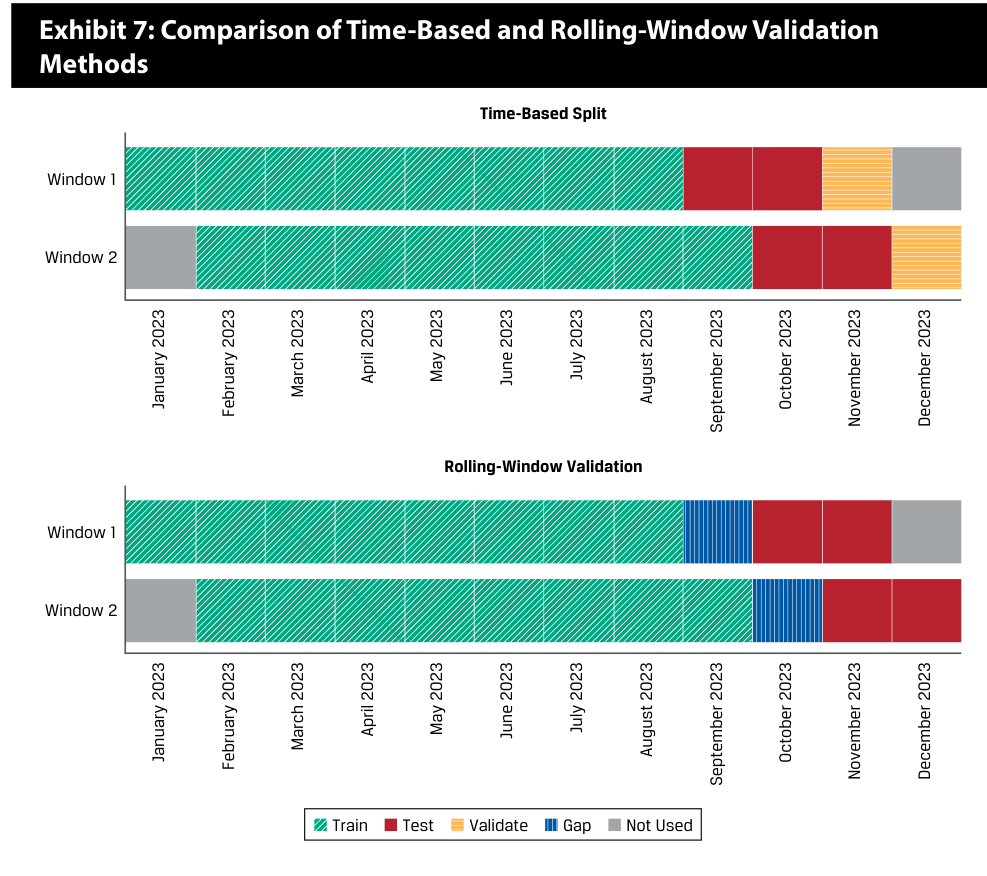
\includegraphics[width=0.8\linewidth]{002_figs/011_Module_11/11.2-Time vs Rolling.png}
	\caption{Time-Based Split vs. Rolling-Window Validation}
	\label{fig:time_vs_rolling}
\end{figure}

\subsection{Overfitting vs. Underfitting}
\begin{itemize}
	\item \textbf{Overfitting:} The model learns the training data too precisely, capturing random noise as if it were a true parameter. This leads to extremely low training error but high out-of-sample test error ($Error_{\text{train}} \ll Error_{\text{test}}$).
	\item \textbf{Underfitting:} The model is too simplistic and treats true relationships as noise, failing to learn the underlying structure in the training data.
\end{itemize}

\subsection{Machine Learning Approaches}
Machine learning is classified into four main approaches, summarized in Table~\ref{tab:ml_approaches}:

\begin{table}[!htbp]
\centering
\caption{Comparison of Machine Learning Approaches}
\label{tab:ml_approaches}
\begin{tabular}{p{0.14\linewidth} | p{0.22\linewidth} | p{0.15\linewidth} | p{0.16\linewidth} | p{0.16\linewidth}}
	\toprule
	\textbf{Approach} & \textbf{Description} & \textbf{Applications} & \textbf{Advantages} & \textbf{Limitations} \\
	\midrule
	\textbf{Supervised learning} & Models learn from labeled historical training data where target output is known. & • Spam detection \newline • Stock return prediction \newline • Default classification & • Highly accurate \newline • Well-understood methods & • Labeled data is costly \newline • Fails to generalize to new scenarios \\
	\midrule
	\textbf{Unsupervised learning} & Models analyze unlabeled data to discover hidden structures and groupings. & • Customer segmentation \newline • Anomaly detection \newline • Dimension reduction & • Discovers unexpected patterns \newline • Reduces data dimensionality & • Subjective evaluation \newline • Difficult to interpret results \\
	\midrule
	\textbf{Reinforcement learning} & Models learn by trial-and-error interaction with an environment to maximize rewards. & • Portfolio optimization \newline • Algorithmic execution & • Good for sequential decisions \newline • Adapts to dynamics & • High training time \newline • Sensitive to reward design \\
	\midrule
	\textbf{Deep learning} & Models use multi-layered artificial neural networks to extract abstract patterns. & • Image recognition \newline • NLP & • Automatically extracts features \newline • Models non-linear structures & • "Black box" nature \newline • Requires massive datasets \\
	\bottomrule
\end{tabular}
\end{table}

\subsection{Neural Networks and Generative Models}
\textbf{Neural networks} are computational models inspired by biological brains. A neural network consists of layers of interconnected nodes (neurons):
\begin{itemize}
	\item \textbf{Input layer:} Receives the raw input features (e.g., historical returns, financial ratios).
	\item \textbf{Hidden layers:} Intermediate layers where non-linear data transformations occur. Multiple hidden layers constitute a "deep" neural network.
	\item \textbf{Output layer:} Provides the final classification or predicted continuous value.
\end{itemize}

\begin{figure}[!htbp]
	\centering
	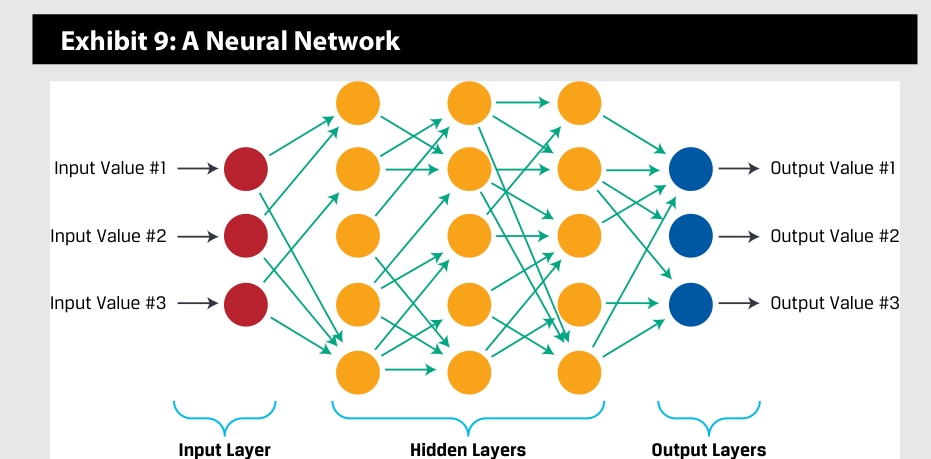
\includegraphics[width=0.7\linewidth]{002_figs/011_Module_11/11.3-Neural Network.png}
	\caption{Structure of an Artificial Neural Network}
	\label{fig:neural_network}
\end{figure}

Training is completed using **backpropagation**:
1. \textbf{Forward pass:} Data flows through the network to generate a prediction.
2. \textbf{Loss calculation:} Computes the error (loss) between the predicted and actual target.
3. \textbf{Backward pass (Backpropagation):} Calculates gradients of the loss function with respect to the network weights.
4. \textbf{Weight update:} Weights are updated slightly in the opposite direction of the gradient using **gradient descent**.
This process is repeated over multiple cycles (**epochs**) until the network converges.

Two advanced generative neural network architectures are:
\begin{itemize}
	\item \textbf{Generative Adversarial Networks (GANs):} Combines a generator network (creates synthetic data) and a discriminator network (evaluates authenticity) in an adversarial loop. Used to generate synthetic financial scenarios for stress-testing.
	\item \textbf{Variational Autoencoders (VAEs):} Compresses inputs into a latent, lower-dimensional space (encoder) and reconstructs them (decoder). Useful for dimensionality reduction and anomaly detection.
\end{itemize}

\vspace{1.5em}

\section{Natural Language Processing and Generative AI}
\label{sec:NLP and Generative AI}

\subsection{Natural Language Processing (NLP)}
\begin{itemize}
	\item \textbf{Text analytics} extracts information and identifies patterns from unstructured text- or voice-based datasets (filings, transcripts, emails, news, etc.).
	\item \textbf{Natural language processing (NLP)} is a subfield at the intersection of computer science, AI, and linguistics focused on analyzing human language.
\end{itemize}
Common applications in finance include sentiment analysis (e.g., parsing earnings call transcripts to assign a positive/negative sentiment rating to detect subtle manager outlooks before analyst rating updates) and monitoring central bank communication (parsing Fed or ECB statements to extract tone shifts on interest rates).

\subsection{Large Language Models (LLMs)}
**Large Language Models (LLMs)**, such as GPT models, represent a significant advancement in generative AI. 
\begin{itemize}
	\item \textbf{Architecture:} Rely on **transformers** to process and capture long-range contextual relationships within textual sequences.
	\item \textbf{Huấn luyện song miền (Dual-domain training):} Sourced via self-supervised learning on massive general corpora (to learn grammar, semantics) and specialized financial corpora (filings, earnings call transcripts to master domain jargon).
	\item \textbf{Tinh chỉnh (Fine-tuning):} Adapted via transfer learning for specialized applications (e.g., text generation, report summarization, financial sentiment analysis).
	\item \textbf{Rủi ro và hạn chế (Risks):} LLMs excel at language prediction but are prone to **hallucinations** (generating false information) and lack numerical calculation capabilities. Over-reliance can result in strategic and regulatory errors. A hybrid model combining automated outputs with human review is recommended.
\end{itemize}

\subsection{Generative AI vs. Traditional Simulations}
**Generative AI** creates new content or scenarios based on representations learned during training. Unlike Monte Carlo simulations (which assume predefined parametric distributions) or bootstrapping (which simply shuffles or resamples historical records), Generative AI learns complex underlying data structures to produce realistic, non-replication-constrained synthetic scenarios.

\vspace{1.5em}

\section{Practice Problems and Solutions}
\label{sec:Practice_Problems_Module_11}
\textcolor{blue}{\textit{Các bài tập ôn tập kèm Lời giải của Module 11 đã được chuyển về Chương 14 (Bài tập ôn tập và Lời giải) ở cuối bản PDF để tiện tra cứu tập trung. Xem bài tập và lời giải tại trang \pageref{sec:app_Problems_M11}.}}
